\resetgraphicspath
\appendtographicspath{{./Introduction/figures}}
\appendtographicspath{{./Chapter 1/figures/} }
\appendtographicspath{{./Chapter 1/islands} }
\appendtographicspath{ {./Chapter 3/figures/erosion/}{./Chapter 3/figures/terrain_representations/}{./Chapter 3/results/}{./Chapter 3/otherPapersRepro/} {./Chapter 3/images/erosion-processes/}}

\chapter{State of the art}

\minitoc

\newpage

\section{Terrain representation}
Terrain refers to the physical features and configuration of a specific area of land. It includes the elevation, slope, and the overall topography, such as mountains, valleys, and plains. Terrain is often used to describe the surface characteristics of the land, focusing on the natural contours and the geographical aspects that define a region's physical form.

While the term "terrain" describes the physical characteristics of land, it does not include the natural elements that shape an area's identity. Elements like vegetation, water bodies, and climatic conditions, such as snow cover, are essential to how we perceive and understand a landscape. Therefore, when discussing procedural generation in virtual environments, "landscape generation" is a more fitting term, as it integrates these natural elements along with the topographical features.

In addition to "terrain generation," other terms such as "landscape generation," "world generation," and "environment generation" can be used to describe the creation of virtual landscapes. These terms are interchangeable and can all refer to the process of generating physical terrain along with natural and artificial elements. However, by convention and for simplicity, the term "terrain generation" is most commonly used in the field. Despite its original focus on the physical features of the land, "terrain generation" has evolved to encompass a broader range of environmental elements, making it a convenient and widely accepted term for describing the comprehensive process of creating virtual environments.

A terrain can be represented in various ways, each of them suited for a given application of which we give an brief overview, more details can be found in \cite{Galin2019}.

\subsection{Elevation models}

\begin{figure}[H]
    \centering
    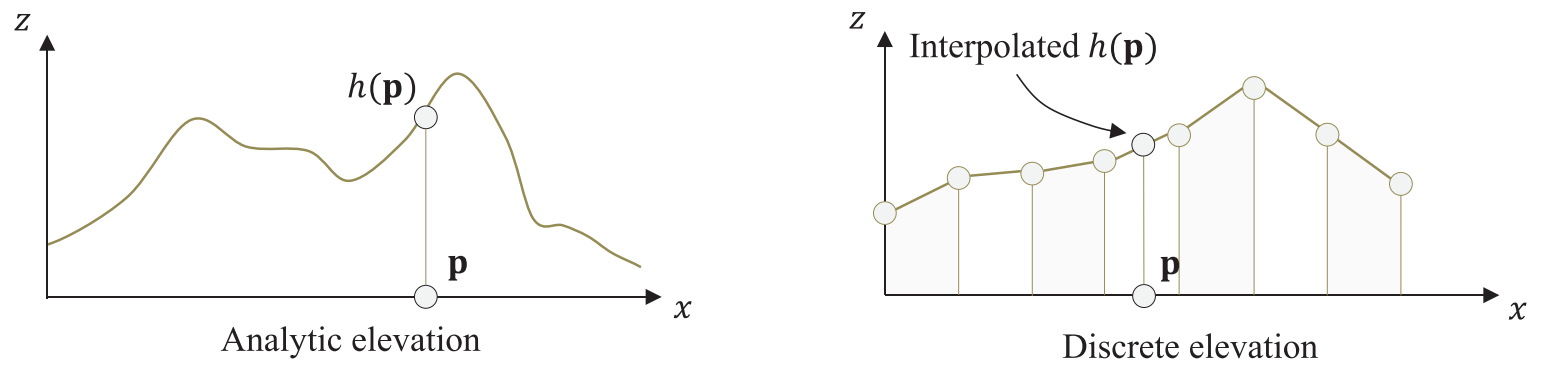
\includegraphics[width = 0.8 \linewidth]{elevation_representation.png}
    \caption{Elevation functions}
    \label{fig:erosion-elevation-representation}
\end{figure}

Elevation models are a fundamental approach in terrain representation, widely used in procedural generation due to their simplicity and efficiency. These models define the terrain as a function $h : \R^2 \to \R$, where each point in a 2D plane is mapped to an elevation value. This approach is particularly effective for representing terrains where the elevation is the only varying factor, such as hills, valleys, and plateaus, and it is best suited for terrains without complex 3D features like overhangs or caves. While we visualize elevation models in three dimensions, they are mathematically considered two-dimensional functions. In the domain of terrain generation, we will name them 2.5D models.

Elevation models are widely used in industries where large-scale terrain representation is crucial. In video games, they provide the foundation for creating vast open-world environments. In geographic information systems (GIS) and remote sensing, height fields are used to represent real-world terrain data, offering a practical means of visualizing and analyzing geographical features. The ability to manipulate and control terrain features procedurally makes elevation models a common choice for applications that require efficient terrain generation and rendering.

They offer a powerful method for representing terrains in procedural generation, combining simplicity with flexibility. While they have limitations in representing complex 3D structures, their efficiency and compatibility with existing algorithms make them indispensable in a variety of applications.

\subsubsection{Implicit height fields}

\begin{wrapfigure}{L}{0.4\textwidth}
    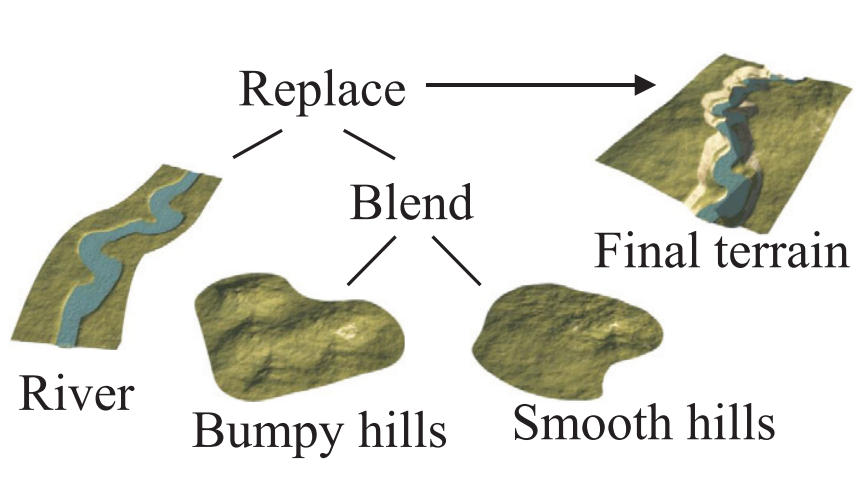
\includegraphics[width=\linewidth]{primitives_representation.png}
    \caption{Primitives composition}
    \label{fig:erosion-primitives-representation}
\end{wrapfigure}

Implicit height fields represent the terrain as a mathematical function that provides a height value at any given point in the domain. These functions can be procedural or closed-form expressions, allowing for compact storage and infinite precision in theory. The elevation function allows for easy manipulation of terrain features, making it ideal for generating terrains that require smooth, continuous surfaces. However, the primary disadvantage is the computational complexity involved in evaluating the function, especially for large or highly detailed terrains. The challenge lies in constructing functions that can realistically represent large-scale terrains with complex landforms.

\subsubsection{Discrete height fields}
Discrete height fields, or explicit height fields, are one of the most prevalent methods for terrain representation. These models consist of a 2D grid where each cell contains a height value, representing the elevation at that point. Height fields are particularly advantageous because they are simple to implement and are directly compatible with many rendering techniques and hardware, but also due to their closeness with image processing, a domain studied for many decades now.

The main advantage of height fields is their ability to handle large datasets efficiently, providing a balance between memory usage and detail. However, they are limited by their inability to represent terrains with overhangs or caves, as each point on the grid can only hold a single elevation value. Additionally, height fields often require interpolation methods, such as bi-linear or bi-cubic interpolation, to reconstruct a continuous surface from the discrete grid points. 

\subsection{Volumetric models}

\begin{figure}[H]
    \centering
    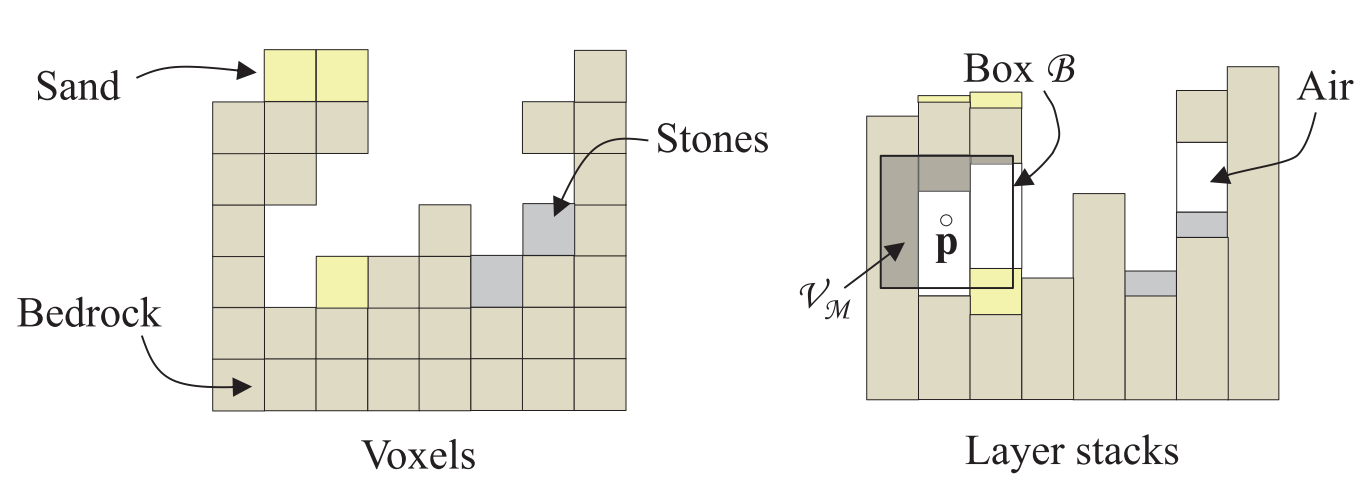
\includegraphics[width = 0.8 \linewidth]{volumetric_representation.png}
    \caption{Volumetric functions}
    \label{fig:erosion-volume-representation}
\end{figure}

Volumetric models represent a more complex approach to terrain modeling, allowing for the depiction of 3D features that go beyond the simple surface-based representation provided by elevation models. These models capture not only the surface of the terrain but also its internal structure, making them ideal for representing terrains with overhangs, caves, and other subsurface features. 

Volumetric models, including layered materials, voxel grids, and implicit models, are essential in applications where terrain complexity and detail are primordial. In geological simulations, these models allow for accurate representation of subsurface structures and processes. Voxel models are widely used in games that require dynamic terrain deformation, providing a rich interactive environment for players. Implicit models are favored in situations where smooth, continuous surfaces are needed [FIND OTHER USE CASES].

\subsubsection{Implicit volumetric models}
Implicit volumetric models describe the terrain's shape and features using an implicit function. The terrain is represented by a mathematical function $f: \R^3 \to \R$ that determines the terrain surface by evaluating to an isovalue, often zero. This function provides a continuous representation of the terrain, with points inside the terrain returning positive values and while points in the air evaluate to negative values. It allows for the seamless representation of complex terrain features, including caves, overhangs, and varying geological structures, which are impossible to represent with  elevation models.

One of the key advantages of implicit models is their ability to produce smooth surfaces without the need for discrete polygonal meshes, which can result in realistic and natural-looking terrains. However, the computational complexity of evaluating the implicit function, especially for large terrains, can be a significant drawback. Additionally, converting an implicit surface into a mesh for rendering can be challenging and resource-intensive. \cite{Araujo2015} 

\subsubsection{Layered models}
Layered models are a type of volumetric representation that encode different material layers within the terrain and are defined by a function $\mu : \R^3 \to \material$, where $\material$ denotes the material type at any given point in 3D space. This allows for a detailed representation of the terrain's internal composition, which can be crucial for applications requiring realistic geological simulations. Each layer is defined by its thickness or elevation, and multiple layers can be stacked to represent complex geological formations. These layers might include materials like bedrock, sand, soil, or water, each contributing to the overall structure of the terrain. Layered models are particularly useful in simulations that involve processes like erosion or sedimentation, where the interaction between different material layers affects the physical process.

The primary advantage of layered models is their ability to represent a stratified terrain with distinct material properties, which can be manipulated individually. This makes them well-suited for simulations that require detailed geological accuracy. However, they are more complex to implement than simple elevation models and require additional computational resources to manage the interactions between layers. 


\subsubsection{Voxel grid models}
Voxel grids are a common method for representing 3D terrains in procedural generation, offering the ability to capture complex internal structures and features that are difficult or impossible to represent with surface-based models. In a voxel grid, the 3D space is divided into a regular grid of small, cube-shaped elements called voxels (volumetric pixels). Each voxel holds information about the material or properties of the terrain at that specific point in space. This approach allows for detailed modeling of features such as caves, tunnels, overhangs, and intricate underground networks. The regular grid structure allows for the use of image processing-oriented algorithms.

There are three primary types of voxel grids used in terrain representation: binary voxel grids, material voxel grids and density voxel grids. Each has distinct characteristics, advantages, and limitations, making them suitable for different applications. 

\subsubsubsection{Binary voxel grids}
Binary voxel grids are the simplest form of voxel representation. In these grids, defined $f: \R^3 \to [0, 1]$, each voxel is either "filled" or "empty," representing the presence or absence of material. This binary state is typically represented by a 1 (filled) or 0 (empty). Binary voxel grids are straightforward to implement and require much less memory compared to more complex voxel representations, making them ideal for applications where the primary concern is whether a space is occupied or not.

The simplicity of binary voxel grids is one of their main advantages. They are easy to understand and visualize, with each voxel requiring only a single bit of information to represent its state. Additionally, because only a binary state is stored, these grids can be memory-efficient when combined with compression techniques like Sparse Voxel Octrees (SVOs) \cite{Laine2010} or voxel Directed Acyclic Graphs (DAG) \cite{Villanueva2017,Careil2020}. The simplicity of the data structure also allows for quick processing, making binary voxel grids suitable for real-time applications where performance is required. However, the binary nature of these grids limits their ability to represent variations in material density or properties, or even smoothness, resulting in less detailed terrain models. This can lead to hard, blocky edges in the terrain, which may appear unnatural without additional smoothing or processing.

\subsubsubsection{Material voxel grids}
Material voxel grids, defined as $\mu: \R^3 \to \material$, are commonly used in applications where simple occupancy information is sufficient. For example, voxel-based games like Minecraft utilize material grids to create terrains composed of solid blocks with clear boundaries. These grids are also employed in scientific simulations where the primary concern is the presence or absence of materials, rather than detailed material properties.

\subsubsubsection{Density voxel grids}
Finally, density voxel grids allow each voxel to store a range of values, representing varying degrees of material presence with $f: \R^3 \to \R$. Instead of a simple discrete state, a density voxel grid assigns a continuous value to each voxel, which can represent material density, opacity, or other properties. This added complexity enables density voxel grids to represent subtle variations in terrain, such as gradual changes in material density or smooth transitions between solid and empty spaces, allowing for more realistic and natural-looking terrain models.

% The use of density voxel grids results in soft transitions and smooth surfaces, reducing the blockiness typically associated with binary voxel grids. They are versatile and can represent not only solid terrain but also phenomena like fog, fluid densities, or temperature gradients. However, the increased detail and realism come at the cost of greater complexity. Density voxel grids require more memory and computational power, making them more challenging to implement and manage. The additional data and processing required can also lead to slower performance, particularly in real-time applications.

Density voxel grids are often used in high-fidelity simulations where detail and realism are essential. They are found in applications such as medical imaging, scientific visualizations, and advanced terrain modeling for films and visual effects. These grids are also employed in procedural terrain generation systems that require smooth and natural transitions between different terrain features, such as caves, cliffs, and eroded landscapes.



% Procedural terrain generation has been heavily studied for the last 40 years \cite{Galin2019}. Researches in this topic try to find new solutions to compromise between realism, user control and efficiency \cite{Gain2009}. Using fractal noise parametrized to resemble real landscape has been an important first step \cite{Musgrave1989} as it's a fast and light solution to generate procedurally the appearance of mountains. The lack of user control pushed newer works toward the use of controlled noise by including real DEM in the process through learning \cite{Kapp2020}, while the rise of deep learning technologies gave higher control to the user through sketches \cite{Guerin2017, Talgorn2018}.

% All the algorithms aim to reproduce plausible relief in terrestrial landscapes, mostly limited to alpine landscapes, but a lack of research can be found in almost all other biomes \cite{Smelik2014}. Underwater landscapes generation, for example, has been almost completely absent from literature for many reasons: the difficulty of accessing the area, the lack of visibility under water and the complex physics of underwater geology and biology make the algorithms adapted for this environment scarce. 

% While stochastic noise may be sufficient to model coarsely the ocean floor \cite{Mareschal1989}, this process won't cover areas with the biggest biomass, near shallower waters such as near coasts and islands. These areas, that represent a very small portion of the oceanic surface, are much more complex as many interactions between biolife, air and water are in action.

% Due to the impossibility to observe the large-scale and the small-scale of underwater environments, some works related to geology model large structures like the profile shape of the coral reef \cite{Bosscher1992}, simulate its surface growth \cite{Li2021}, or use procedural algorithms for single coral colonies' growth simulation \cite{Abela2015}. We however don't have a mix of the different scales, and neither methods take into account the environment such as the topography or the interaction of different terrain features. This is mainly due to the fact that the evolution time for each scale varies from a span of weeks to thousands of years.

% \subsection{Vector modeling}

% Recent works have been presenting "feature tools" to correct landscapes from unaccurate DEM (2.5D) using vector-based features that modifies the geometry of the ground and water bodies to fit thir respective 2D satellite images, by explicitely defining the position of natural features like rivers and mountains \cite{Ketabchi2016}. Visible 3D features like vegetation and buildings can also be added in the final result as meshes affected to a single point. This leads to sketch-based applications where features are represented like topographic maps. This solution allows for the manipulation of an existing terrain, guided by a real-world satellite image, but lacks the possibility to completely generate an unseen landscape or for the terrain features to interact between them. Feature tools have been proposed to generate terrains from scratch \cite{Smelik2010a}, but usually require to define in advance the interactions between each feature like a automatically displaying a bridge when a river crosses a road.

% \subsubsection{Implicit modeling}
% ...
% \subsubsection{Diffusion models}
% ...







\section{Procedural methods for terrain generation}

Procedural terrain generation has been heavily studied for the last 40 years \cite{Galin2019}. Researches in this topic try to find new solutions to compromise between realism, user control and efficiency \cite{Gain2009}. Using fractal noise parametrized to resemble real landscape has been an important first step \cite{Miller1986} as it's a fast and light solution to generate procedurally the appearance of mountains. Erosion simulation on synthetic terrains has quickly been introduced to improve plausibility, first as \textit{ad hoc} geometric-based formulations \cite{Kelley1988,Musgrave1989} for fast results, then relying on physically-based formulation \cite{Neidhold2005} using more computing power for realism. The lack of user control pushed newer works toward the use of controlled noise by including real DEM in the process through learning \cite{Kapp2020} to prioritize plausibility, while the rise of deep learning technologies gave higher control to the user through sketches \cite{Guerin2017, Talgorn2018}.

% All the algorithms aim to reproduce plausible relief in terrestrial landscapes, mostly limited to alpine landscapes, but a lack of research can be found in almost all other biomes \cite{Smelik2014}. Underwater landscapes generation, for example, has been almost completely absent from literature for many reasons: the difficulty of accessing the area, the lack of visibility under water and the complex physics of underwater geology and biology make the algorithms adapted for this environment scarce. 

\subsection{Noise functions}
% Noise functions

\subsection{Erosion simulation}
% Erosion simulation

\begin{figure}[H]
    \centering
    \begin{minipage}{0.45\linewidth}
        % \centering
        \autofitgraphics[]{erosionCellularHawick2014.png, erosionHydraulicBenes2006.png}
        % 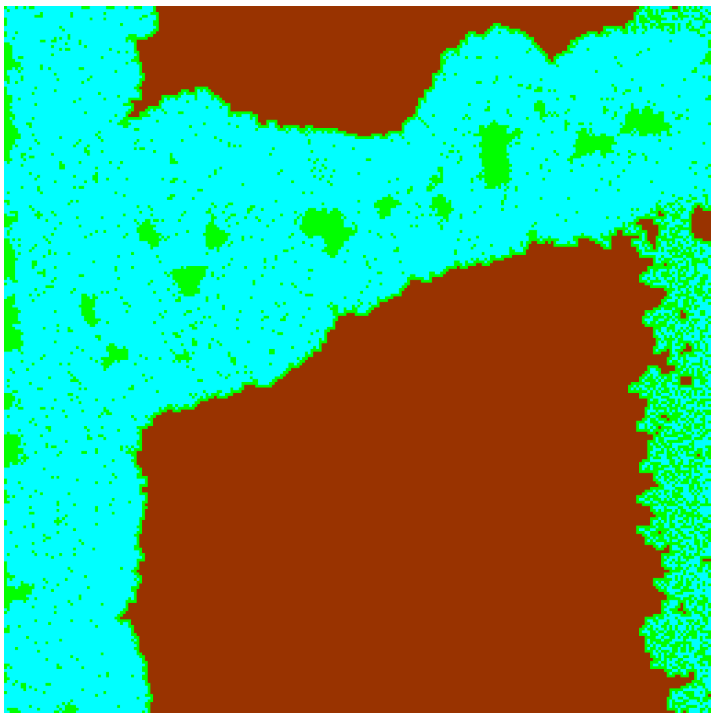
\includegraphics[width = 0.44 \linewidth]{erosionCellularHawick2014.png}
        % 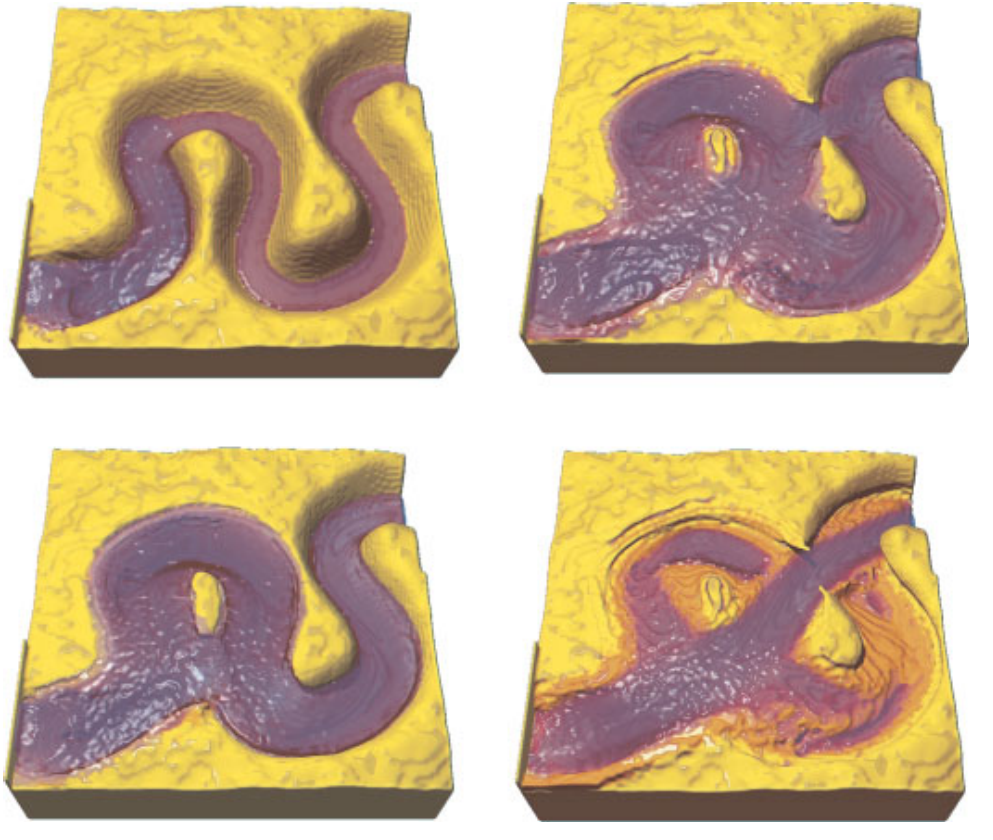
\includegraphics[width = 0.44 \linewidth]{erosionHydraulicBenes2006.png}
    \end{minipage}
    \begin{minipage}{0.45\linewidth}
        % \centering
        % \autofitgraphics[]{erosionHydraulicSchott2023_2.png, erosionRoudier1993.png}
        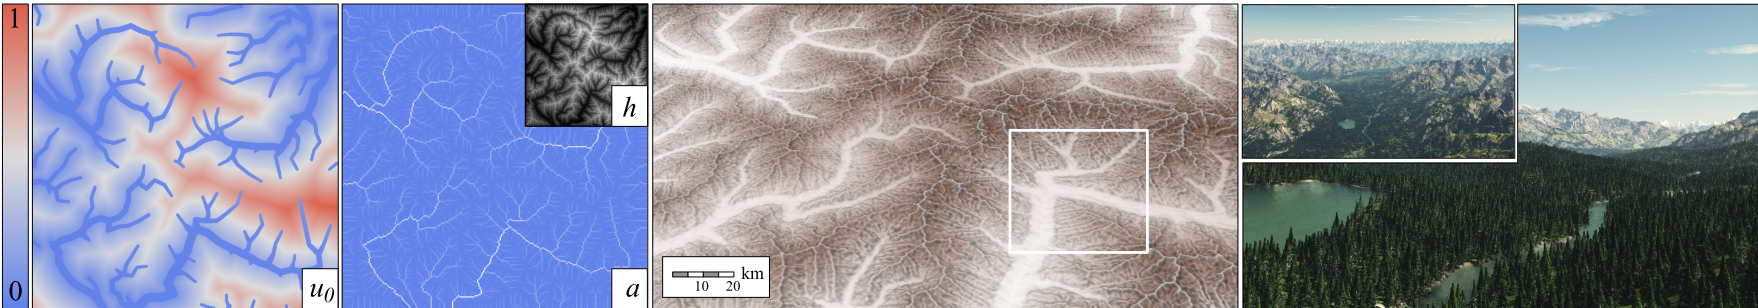
\includegraphics[width = \linewidth]{erosionHydraulicSchott2023_2.png}
        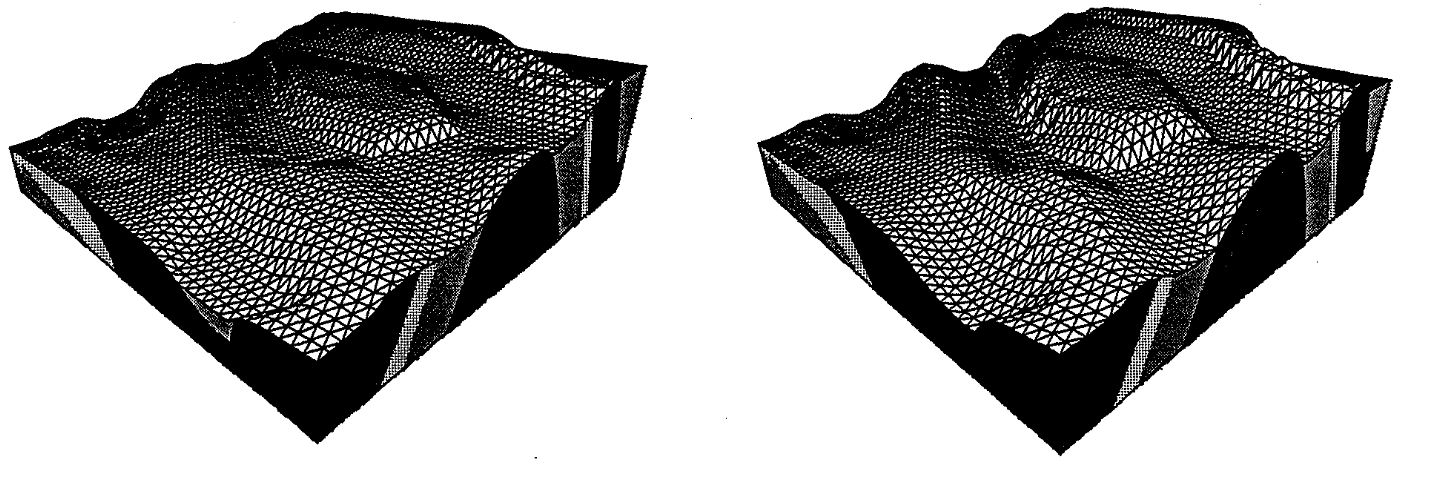
\includegraphics[width = \linewidth]{erosionRoudier1993.png}
    \end{minipage}
    \caption{Four examples from \cite{Hawick2014}, \cite{Benes2006}, \cite{Schott2023} and \cite{Roudier1993}.}
    \label{fig:coral-island-erosion-example}
\end{figure}

While noise functions generate random, natural-looking terrain, they often fail to capture the physical processes that shape real landscapes over time. To address this limitation, erosion simulations model how natural forces such as water flow and gravity wear down terrain features, creating valleys, river networks, and other detailed landforms. These simulations are particularly effective at representing mountainous landscapes, where erosion gradually sculpts the terrain over long periods of time, typically on the scale of hundreds to millions of years.

% Erosion simulations often use models like the Stream Power Law to describe how water erodes higher elevations and deposits sediment in lower areas. The rate of erosion depends on factors such as slope steepness and water flow, with steeper slopes and greater water volumes leading to faster erosion. Over time, these processes create detailed and realistic terrain features like river valleys and erosion channels.
Erosion models are iterative, simulating the gradual shaping of landscapes by continuously balancing forces like erosion and uplift, as seen in the work of \cite{Cordonnier2016,Cordonnier2017a}. Their model simulates how tectonic forces uplift terrain, which is then eroded away over thousands of years. Similarly, \cite{Schott2023} and \cite{Tzathas2024} refined the Stream Power Law to generate realistic slopes and ridges through these long-term geological processes.

Despite their effectiveness in modeling large-scale terrain evolution, erosion simulations are limited when it comes to representing environments that are shaped by dynamic biological processes. A solution to this challenge is to alternate a geological simulations and an ecosystem simulations to capture the feedback of the two systems at the cost of increasing drastically the computation time \cite{Cordonnier2017b}. Coral reefs, for instance, grow and adapt to changing environmental conditions on a much shorter timescale than geological erosion. While erosion models simulate terrain changes over millennia, coral growth responds more dynamically to factors like water depth, light availability, and temperature on scales ranging from years to decades. These biological factors are difficult to incorporate into traditional erosion models, which are designed to simulate the slow, steady forces of water and gravity. [CITATION DEADWOOD DE GUERIN 2024] [ADD DETAILS, WHAT IT CAN OR CAN'T DO, PROBLEM OF TIME].

% Our approach builds on the concept of terrain evolution by integrating the geological and biological dynamics that shape coral reef islands. Instead of focusing solely on erosion, which is primarily a surface-level process, we model the subsidence of volcanic islands over geological time and the simultaneous growth of coral reefs that adapt to the changing sea levels. Coral reefs must grow upward to remain within the photic zone, a process that unfolds on shorter timescales than those captured by standard erosion simulations. Furthermore, we introduce wind deformation to simulate the effects of environmental forces like wind and waves, which reshape the island's structure. This combination of long-term geological processes and short-term biological responses provides a more comprehensive simulation of coral reef island formation, capturing both the slow subsidence of volcanic landmasses and the rapid adaptability of coral ecosystems.

\subsection{Sketching}
% Sketching

% \begin{figure}[ht]
% 	\centering
% 	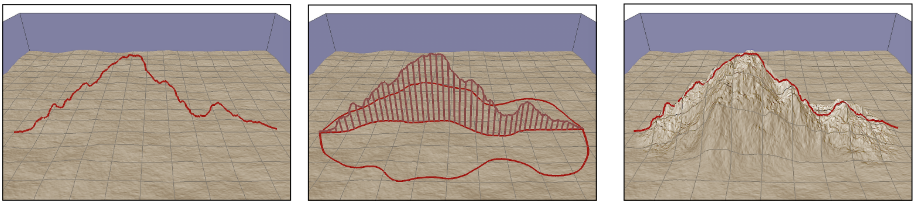
\includegraphics[width = 0.45 \linewidth]{sketchingGain2009.png}
%     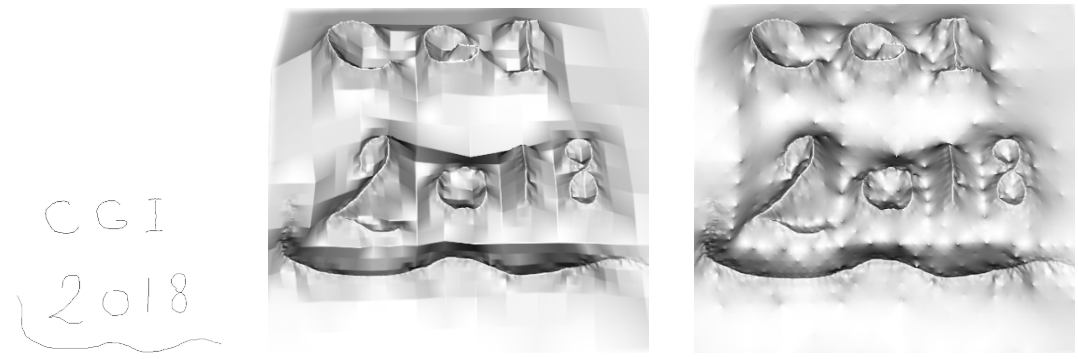
\includegraphics[width = 0.45 \linewidth]{sketchingTalgorn2018.png}
%     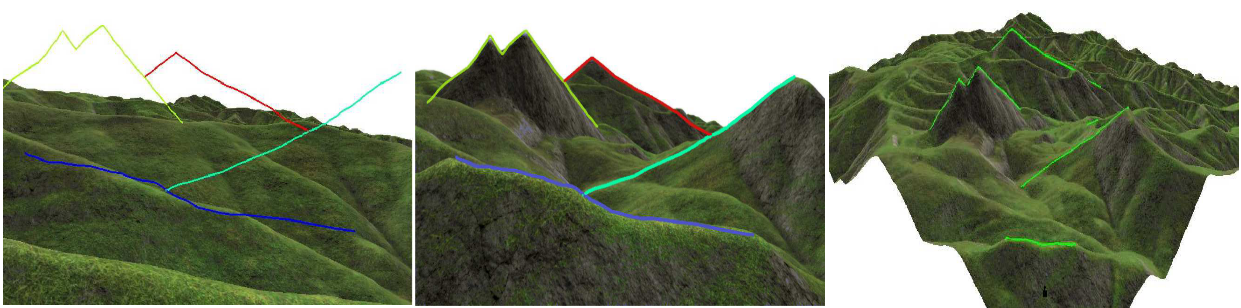
\includegraphics[width = 0.45 \linewidth]{sketchingTasse2014.png}
%     \caption{From \cite{Gain2009}, \cite{Talgorn2018}, \cite{Tasse2014}}
%     \label{fig:coral-island-sketching-examples}
% \end{figure}

In procedural terrain generation, sketch-based approaches allow users to directly interact with and shape landscapes through intuitive sketching interfaces. These methods enable users to define key terrain features such as mountains, valleys, and coastlines by drawing them in a two-dimensional canvas, which are then translated into 2.5D terrains. Sketching provides a high level of artistic control, making it especially useful in creative applications such as video games and simulations, where user-defined terrain features are prioritized.

\wrapFigR{sketchingTasse2014-vertical-s.png}{0.25}{fig:sketching-tasse-2014}
{From \cite{Tasse2014}, the first person view constraint allows for a sketching of mountains by a single stroke.}

Sketch-based systems offer great flexibility, allowing users to directly define specific elements of the landscape according to their needs or preferences. For instance, \citep{Gain2009} introduced a multi-perspective sketching system that allows users to generate detailed landscapes by sketching from different angles. This method provides more control over the terrain's shape than traditional noise-based generation methods. Similarly, \citep{Tasse2014} explored sketching from the player's viewpoint, allowing users to dynamically define height information from within the virtual environment, creating an interactive terrain design experience.

\wrapFigL{sketchingGain2009-vertical-s.png}{0.25}{fig:sketching-gain-2009}
{From \cite{Gain2009}, a mountain is generated by a top-view shape and a height function}

Sketching has also been extended to geological modeling. \citep{Patel2021} proposed a system where users can interactively model underground layers by sketching subsurface structures. This provides a powerful tool for geologists and designers who need to model complex, multi-layered terrains, offering more control over both the surface and the subsurface.

In our work, we leverage the flexibility of sketching to define the key features of coral reef islands, such as the island shape, lagoons, and coral reefs, in a vectorized format. This is particularly important for modeling underwater and island landscapes, where these features are not simply surface elements but part of an evolving geological structure. By using sketches, we retain the semantic information of where the island and coral regions are located, which allows us to later apply our simplified model of Darwin's subsidence theory.

% \wrapFigL{sketchingTalgorn2018.png}{0.25}{fig:sketching-taglorn-2018}{From \cite{Talgorn2018}, a mountain is generated by a top-view shape and a height function [Need to change the image to vertical]}

Rather than focusing on detailed long-term or short-term evolution, our method adapts sketching to the unique requirements of island and underwater landscapes. Once the user defines the terrain layout through sketching, we apply a simplified subsidence model, where the volcanic island gradually sinks and coral reefs grow in response, remaining close to the water surface. This process provides a framework for simulating the evolution of the landscape in a geologically plausible manner.

The key advantage of sketching in our system is that it combines the artistic control provided by traditional sketching methods with the ability to handle the geological processes specific to coral reef islands. By preserving the vectorized information from the sketch, we can accurately place and evolve features like lagoons and coral reefs, ensuring that the resulting terrain reflects both the user's design intent and the geological dynamics at play.

[NEED TO ADD AT LEAST \cite{Talgorn2018}]

